\documentclass[12pt]{chmullighw}
\usepackage{tikz}
\usepackage{tikz-qtree}
\usepackage{algorithm2e}
\usetikzlibrary{shapes,chains,fit,shapes,matrix}


% info for header block in upper right hand corner
\name{Chris Mulligan}
\uni{clm2186}
\class{COMS3137 Data Structures \& Algorithms}
\professor{Hershkop}
\assignment{Theory 3}
\duedate{October 27, 2013}

\lstset{language=Java, numbers=none, frame=l, captionpos=n}
\begin{document}
\problemlist{Theory 3} %Give us a nice big title
\begin{enumerate}

\item \begin{enumerate} \renewcommand{\labelenumii}{\alph{enumii}.}
    \item Chaining:

        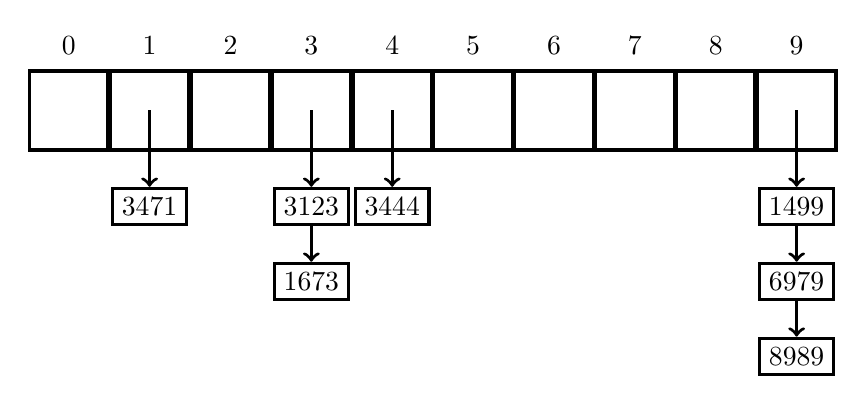
\begin{tikzpicture}
        \tikzstyle{every path}=[very thick]

        \edef\sizetape{1cm}
        \tikzstyle{ht}=[draw,minimum size=\sizetape]
        \tikzstyle{num}=[draw=none]
        \tikzstyle{value}=[draw]

        \begin{scope}[start chain=1 going right,node distance=-0.15mm]
        \foreach \x in {0, 1,...,9} {
            \node [on chain=1,ht] (\x) {};
        };
        \end{scope}

        %label the cells above
        \foreach \x in {0, 1,...,9} {
            \node [num,yshift=.3cm] at (\x.north) (\x_label) {$\x$};
        };

        \node[value, yshift=-.7cm] at (1.south) (3471) {3471};
        \draw[->] (1.center) -- (3471.north);

        \node[value, yshift=-.7cm] at (3.south) (3123) {3123};
        \draw[->] (3.center) -- (3123.north);
        \node[value, yshift=-.7cm] at (3123.south) (1673) {1673};
        \draw[->] (3123.south) -- (1673.north);

        \node[value, yshift=-.7cm] at (4.south) (3444) {3444};
        \draw[->] (4.center) -- (3444.north);
          
        \node[value, yshift=-.7cm] at (9.south) (1499) {1499};
        \draw[->] (9.center) -- (1499.north);
        \node[value, yshift=-.7cm] at (1499.south) (6979) {6979};
        \draw[->] (1499.south) -- (6979.north);
        \node[value, yshift=-.7cm] at (6979.south) (8989) {8989};
        \draw[->] (6979.south) -- (8989.north);
        \end{tikzpicture}

    \item Linear Probing:

        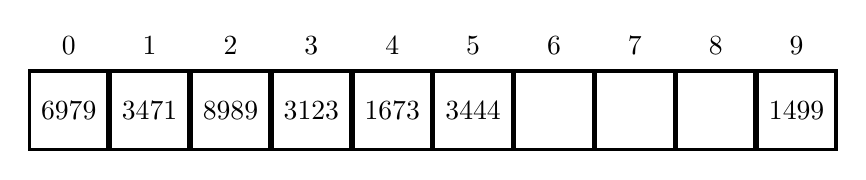
\begin{tikzpicture}
        \tikzstyle{every path}=[very thick]

        \edef\sizetape{1cm}
        \tikzstyle{ht}=[draw,minimum size=\sizetape]
        \tikzstyle{num}=[draw=none]
        \tikzstyle{value}=[draw]

        \begin{scope}[start chain=1 going right,node distance=-0.15mm]
        \node [on chain=1,ht] (0) {6979};
        \node [on chain=1,ht] (1) {3471};
        \node [on chain=1,ht] (2) {8989};
        \node [on chain=1,ht] (3) {3123};
        \node [on chain=1,ht] (4) {1673};
        \node [on chain=1,ht] (5) {3444};
        \node [on chain=1,ht] (6) {};
        \node [on chain=1,ht] (7) {};
        \node [on chain=1,ht] (8) {};
        \node [on chain=1,ht] (9) {1499};
        \end{scope}

        %label the cells above
        \foreach \x in {0, 1,...,9} {
            \node [num,yshift=.3cm] at (\x.north) (\x_label) {$\x$};
        };
        \end{tikzpicture}

    \item Quadratic Probing:

        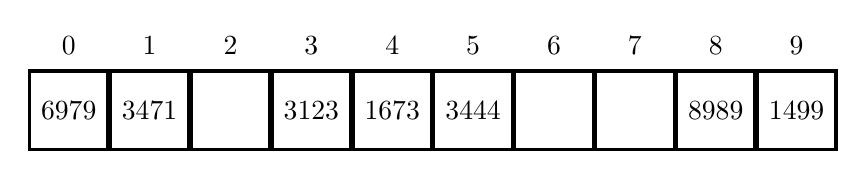
\begin{tikzpicture}
        \tikzstyle{every path}=[very thick]

        \edef\sizetape{1cm}
        \tikzstyle{ht}=[draw,minimum size=\sizetape]
        \tikzstyle{num}=[draw=none]
        \tikzstyle{value}=[draw]

        \begin{scope}[start chain=1 going right,node distance=-0.15mm]
        \node [on chain=1,ht] (0) {6979};
        \node [on chain=1,ht] (1) {3471};
        \node [on chain=1,ht] (2) {};
        \node [on chain=1,ht] (3) {3123};
        \node [on chain=1,ht] (4) {1673};
        \node [on chain=1,ht] (5) {3444};
        \node [on chain=1,ht] (6) {};
        \node [on chain=1,ht] (7) {};
        \node [on chain=1,ht] (8) {8989};
        \node [on chain=1,ht] (9) {1499};
        \end{scope}

        %label the cells above
        \foreach \x in {0, 1,...,9} {
            \node [num,yshift=.3cm] at (\x.north) (\x_label) {$\x$};
        };
        \end{tikzpicture}

    \item Second hash function $h_2(x) = 7 - (x \mod 7)$:

        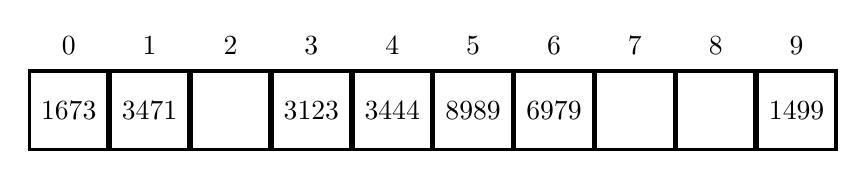
\begin{tikzpicture}
        \tikzstyle{every path}=[very thick]

        \edef\sizetape{1cm}
        \tikzstyle{ht}=[draw,minimum size=\sizetape]
        \tikzstyle{num}=[draw=none]
        \tikzstyle{value}=[draw]

        \begin{scope}[start chain=1 going right,node distance=-0.15mm]
        \node [on chain=1,ht] (0) {1673};
        \node [on chain=1,ht] (1) {3471};
        \node [on chain=1,ht] (2) {};
        \node [on chain=1,ht] (3) {3123};
        \node [on chain=1,ht] (4) {3444};
        \node [on chain=1,ht] (5) {8989};
        \node [on chain=1,ht] (6) {6979};
        \node [on chain=1,ht] (7) {};
        \node [on chain=1,ht] (8) {};
        \node [on chain=1,ht] (9) {1499};
        \end{scope}

        %label the cells above
        \foreach \x in {0, 1,...,9} {
            \node [num,yshift=.3cm] at (\x.north) (\x_label) {$\x$};
        };
        \end{tikzpicture}

\end{enumerate}


\item If in advance you knew the contents of a hash table you could potentially
avoid a collision, but it would be incredibly inefficient. You'd have to effectively
calculate hashes and determine if they collided before creating the actual table.
Then if they did ever collide you could switch table size, or hash function, to
avoid the collision. However ultimately you'd end up doing substantially more work.

\newpage
\item Assuming this is a min heap, such that every parent is smaller than both
of its children.

%\Tree[.23 ]

%\Tree[.23 [.25 ]  \edge[draw=none];[.{} ] ]
After 23, 25, 14: \\
\Tree[.14 [.25 ] [.23 ] ]

%\Tree[.14 [.25 [.27 ] \edge[draw=none];[.{} ] ]
%          [.23 ] ]

%\Tree[.14 [.19 [.27 ] [.25 ] ]
%          [.23 ] ]
After 23, 25, 14, 27, 19, 18: \\
\Tree[.14 [.19 [.27 ] [.25 ] ]
          [.18 [.23 ] \edge[draw=none];[.{} ] ] ]

%\Tree[.14 [.19 [.27 ] [.25 ] ]
%          [.18 [.23 ] [.21 ] ] ]

%\Tree[.14 [.19 [.27 [.28 ] \edge[draw=none];[.{} ] ]
%               [.25 ] ]
%          [.18 [.23 ] [.21 ] ] ]
After 23, 25, 14, 27, 19, 18, 21, 28, 24: \\
\Tree[.14 [.19 [.24 [.28 ] [.27 ] ]
               [.25 ] ]
          [.18 [.23 ] [.21 ] ] ]

%\Tree[.14 [.19 [.24 [.28 ] [.27 ] ]
%               [.22 [.25 ] \edge[draw=none];[.{} ]] ]
%          [.18 [.23 ] [.21 ] ] ]

%\Tree[.14 [.19 [.24 [.28 ] [.27 ] ]
%               [.20 [.25 ] [.22 ] ] ]
%          [.18 [.23 ] [.21 ] ] ]
After 23, 25, 14, 27, 19, 18, 21, 28, 24, 22, 20, 17: \\
\Tree[.14 [.19 [.24 [.28 ] [.27 ] ]
               [.20 [.25 ] [.22 ] ] ]
          [.17 [.18 [.23 ] \edge[draw=none];[.{} ] ]
               [.21 ] ] ]

%\Tree[.14 [.19 [.24 [.28 ] [.27 ] ]
%               [.20 [.25 ] [.22 ] ] ]
%          [.17 [.18 [.23 ] [.24 ] ]
%               [.21 ] ] ]

%\Tree[.14 [.19 [.24 [.28 ] [.27 ] ]
%               [.20 [.25 ] [.22 ] ] ]
%          [.17 [.18 [.23 ] [.24 ] ]
%               [.21 [.26 ] \edge[draw=none];[.{} ] ] ] ]
Final:\\
\Tree[.14 [.19 [.24 [.28 ] [.27 ] ]
               [.20 [.25 ] [.22 ] ] ]
          [.15 [.18 [.23 ] [.24 ] ]
               [.17 [.26 ] [.21 ] ] ] ]

\newpage
\item Let $l$ be the number of leaves, $n$ the total number of nodes, and $n_2$
as the number of nodes of degree 2. Every node has exactly 1 parent, except the
root. We shall prove $n_2 = l - 1$.

If $n = 1$ we only have a root, which is a leaf. $l$ = 1, $n_2$ = 0. \checkmark

Adding a node to a tree already displaying exhibiting this property, there are two cases:
\begin{itemize}
\item If it's the first child of a former leaf, we add increment $l$ for the new
node, but decrement $l$ because the former leaf is now degree 1. The degree of the grandparent, and all other nodes, is unchanged, so $n_2$ is unchanged. $l +1 -1 = l$, $n_2\prime = n_2$
\checkmark
\item If it's the second child of a former leaf, then both $n_2$ and $l$ are
incremented by one, and since $n_2 = l -1$ adding 1 to each side, $n_2 + 1 = (l + 1) - 1$, the equality still holds. \checkmark
\end{itemize}


\item
\tikzset{sibling distance=18pt}

a) \Tree[.18 ]
\hskip .8in
b) \Tree[.18   [.3 ]   \edge[draw=none];[.{} ] ]
\hskip .8in
c) \Tree[.18   [.3 ]
            [.25 ] ]
\hskip .8in
d) \Tree[.18   [.3 [.0 ] \edge[draw=none];[.{} ] ]
                [.25 ] ]

f) \Tree[.18   [.3 [.0 ] \edge[draw=none];[.{} ] ]
                [.25 \edge[draw=none];[.{} ] [.222 ] ] ]
\hskip 1.5in
g) \Tree[.18   [.3
                    [.0 \edge[draw=none];[.{} ] [.2 ] ]
                    \edge[draw=none];[.{} ] ]
                [.25 \edge[draw=none];[.{} ] [.222 ] ] ]

\-\\

h) \Tree[.18   [.3
                    [.0 \edge[draw=none];[.{} ] [.2 ] ]
                    [.11 ] ]
                [.25 \edge[draw=none];[.{} ] [.222 ] ] ]
\hskip 1in
i) \Tree[.18  [.3
                    [.0 \edge[draw=none];[.{} ] [.2 ] ]
                    [.11 \edge[draw=none];[.{} ] [.12 ] ] ]
                [.25 \edge[draw=none];[.{} ] [.222 ] ] ]

\-\\

j) \Tree[.18  [.3
                    [.0 \edge[draw=none];[.{} ] [.2 ] ]
                    [.11 \edge[draw=none];[.{} ] [.12 ] ] ]
                [.25
                    \edge[draw=none];[.{} ]
                    [.222 [.34 ] \edge[draw=none];[.{} ] ] ] ]
\hskip .5in
k) \Tree[.18  [.3
                    [.0 \edge[draw=none];[.{} ] [.2 ] ]
                    [.11 \edge[draw=none];[.{} ] [.12 ] ] ]
                [.25
                    \edge[draw=none];[.{} ]
                    [.222
                        [.34 [.30 ] \edge[draw=none];[.{} ] ]
                        \edge[draw=none];[.{} ] ] ] ]

\-\\

l) Final: \Tree[.18  [.3
                    [.0 \edge[draw=none];[.{} ] [.2 ] ]
                    [.11 \edge[draw=none];[.{} ] [.12 ] ] ]
                [.25
                    \edge[draw=none];[.{} ]
                    [.222
                        [.34 [.30 ] [.40 ] ]
                        \edge[draw=none];[.{} ] ] ] ]

\-\\

Pre-Order: 18, 3, 0, 2, 11, 12, 25, 222, 34, 30, 40

Post-Order: 2, 0, 12, 11, 3, 30, 40, 34, 222, 25, 18

In-order: 0, 2, 3, 11, 12, 18, 25, 30, 34, 40, 222

\item First, set the root node's depth to 0. For each node set their children's
depth to the node's depth + 1. Then recursively call the same routine on each of
the children.

This is \BigO{n} because every node is touched once when its depth is updated,
and once to get all its children. With clever programming that could be reduced
to only once, but both cases are \BigO{n}.

\item  \hskip 1in

\begin{algorithm}[H]
\SetAlgoNoLine
\KwData{Tree T}
\KwResult{A \BigO{n} algorithm for non-recursively in-order traversing a binary tree.}

create stack\;
current = root\;
\While{current is not null or stack is not empty}{
    \If(\tcc*[h]{pop from the stack, and head right}){current is null}{
        current = stack.pop\;
        process current\;
        current = current.right\;
    }
    \If(\tcc*[h]{push onto stack and proceed left}){current is not null}{
        push current onto stack\;
        current = current.left\;
    }
}
\end{algorithm}

This algorithm is \BigO{n} because each node is only touched twice, once when
it is pushed onto the stack, and once when it's popped off and processed. 

\item 
Initial: 
\Tree[.14   [.4 [.2 ] [.13 ]  ]
            [.15 \edge[draw=none];[.{} ] [.18 [.17 ] [.39 ]]]]

After deleting the root (14), we move smallest on right to root:\\
\Tree[.15   [.4 [.2 ] [.13 ]  ]
            [.18 [.17 ] [.39 ]]]

\item After inserting 2, 1, 4, 5, 9, 10, 11:\\
\Tree[.5  [.2  [.1 ]  [.4 ] ]
          [.10  [.9 ]  [.11 ] ] ]

After inserting 13, 3, 17, 33:\\
\Tree[.5 [.2  [.1 ]
              [.4  [.3  ] \edge[draw=none];[.{} ]  ] ]
  [.13  [.10  [.9 ] [.11 ] ]
        [.17  \edge[draw=none];[.{} ]  [.33 ]  ] ] ]

\newpage
\item B+Tree with M=5, L=7, after inserting: 4, 40, 23, 50, 11, 34, 62, 78, 66, 22, 90, 59, 25, 72, 64, 77, 10, 12.

%\includegraphics{q10.pdf}

\newpage
\item This algorithm will work, called with isSimilar on the root nodes. 

\begin{algorithm}[H]
\SetAlgoNoLine
\KwData{Tree a, Tree b}
\KwResult{Recursively determine if two binary trees have the same shape}
\SetKwProg{Fn}{Function}{ is}{end}

\Fn{isSimilar(node a, node b)}{
    \uIf{a is null and b is null}{
        return true\;
    }
    \uElseIf{a is null and b is not null}{
        return false\;
    }
    \uElseIf{a is not null and b is null}{
        return false\;
    }
    \Else{
        leftSimilar = isSimilar(a.left, b.left)\;
        rightSimilar = isSimilar(a.right, b.right)\;
        return (leftSimilar and rightSimilar)\;
    }
}
\end{algorithm}

The runtime is \BigO{n}, where n is the size of the smaller tree. It must touch
every element in both trees to verify they're equal, hence \BigO{n}.

\item AVL and Splay trees are both binary search trees that use auto balancing to
prevent degenerate cases of unbalanced trees. They go about it in different ways.

In an AVL tree the tree is balanced whenever a node is inserted or deleted. It
ensures that along the entire insert path no nodes left and right sides have
heights that differ by more than 1. If they do it performs rotations, either single
or double, to bring the tree back into balance. Thus after every insert and delete
it guarantees the left and right sides of every node will have similar heights.
Insert, find, and delete are all \BigO{\log n}. 

A splay tree uses similar rotations, called zig-zigs and zig-zags, to balance the
tree. However splay trees balances on finds, rather than on inserts. Whenever a
node is found, it is rotated to be the root node. By rotating along the way the
tree comes closer into balance. This permits the tree to be quite unbalanced
(even becoming a linked list in the worst case), but for a sequence of finds
and inserts the tree performs with an amortized \BigO{\log n} runtime. In other
words, for any $M$ operations the runtime is \BigO{M\log n}

AVL trees guarantee that the height of the tree is always approximately $\log n$,
however inserts can be slower, and they don't further optimize. Splay trees may
have cases with very large heights, but they guarantee that more recently accessed
nodes are near the top, which helps with real world usage. Further, splay trees
ensure that the overall runtime is no worse than AVL for a large sequence of
operations.

\end{enumerate} %end of questions
\end{document}
